\newpage
\section{Manual de usuario}
\label{anexo:manual_usuario}

En este anexo se ilustra el funcionamiento, la puesta en marcha y el uso del sistema domótico local para la estancia, el cual se ha dividido en las siguientes secciones diferenciadas para facilitar su consulta según el perfil de uso:

\begin{itemize}
    \item \textbf{Manual del Dispositivo (Hardware y Ubicación):} muestra la descripción física de los nodos sensores, su ubicación recomendada y el proceso de encendido de la instrumentación. Está dirigido principalmente al instalador o administrador del sistema.
    \item \textbf{Manual de Acceso y Conexión:} detalla el procedimiento paso a paso para acceder al panel de control desde la red doméstica (Wi-Fi local) y desde redes externas de forma segura (mediante la red privada VPN). Está dirigido tanto al usuario final como al administrador.
    \item \textbf{Manual del Panel de Control (Interfaz Lovelace):} describe la navegación por el cuadro de mandos digital de la habitación, explicando cómo interpretar las lecturas del clima, el nivel de ruido, el estado de los accesos y los históricos de actividad. Está dirigido al usuario final.
    \item \textbf{Manual del Comportamiento Inteligente (Automatizaciones):} explica el funcionamiento automático de la luz de escritorio, los avisos ergonómicos para la mitigación del sedentarismo (alertas Pomodoro), el sistema de alarma de intrusión perimetral y el ahorro de energía en modo noche. Está dirigido al usuario final.
    \item \textbf{Guía de Resolución de Incidencias:} recopila las preguntas frecuentes y los pasos para solucionar problemas comunes de hardware, red o visualización.
\end{itemize}

\subsection{Manual del dispositivo (hardware y ubicación)}
Para que el sistema domótico local funcione correctamente, se asume como requisito previo que el servidor central (la Raspberry Pi 4 que aloja el núcleo del sistema) se encuentra encendido y conectado directamente por cable de red al enrutador doméstico de acceso, ya sea un router, un repetidor o un punto de acceso.

El sistema físico que interactúa con la estancia consta de tres módulos sensores y actuadores inalámbricos, los cuales se describen a continuación (véase la Figura~\ref{fig:usr_nodos}):

\begin{figure}[H]
    \centering
    \begin{subfigure}[b]{0.32\textwidth}
        \centering
        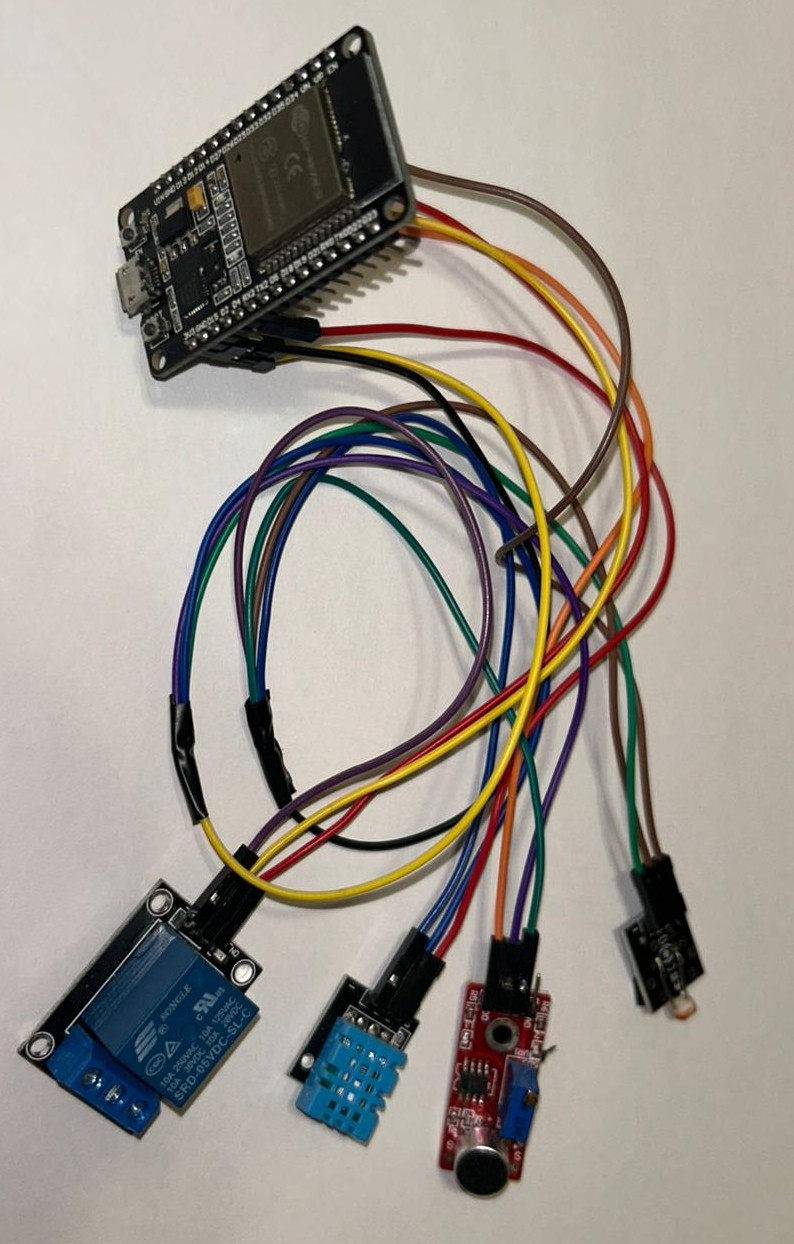
\includegraphics[width=\textwidth]{Img/nodo_ambiente.jpg}
        \caption{Módulo de Ambiente ($N_1$)}
        \label{fig:usr_nodo_amb}
    \end{subfigure}
    \hfill
    \begin{subfigure}[b]{0.32\textwidth}
        \centering
        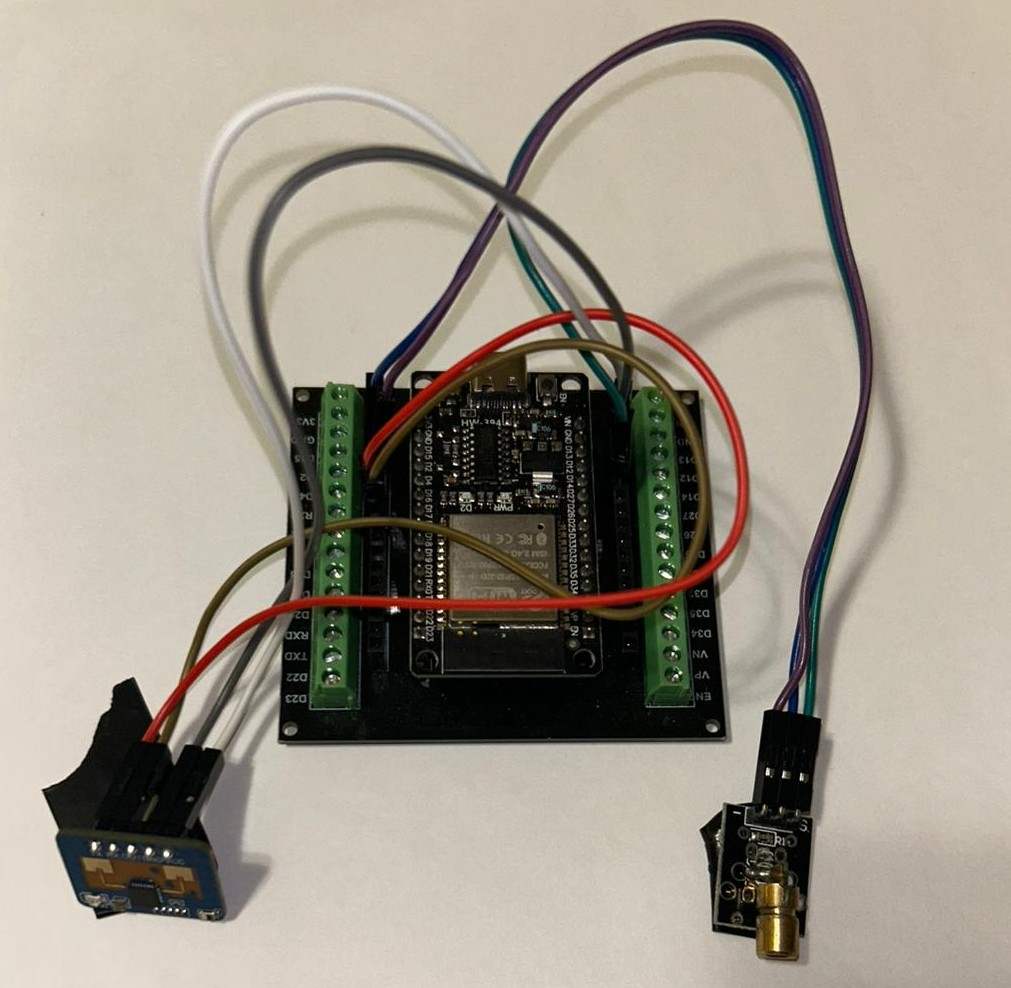
\includegraphics[width=\textwidth]{Img/nodo_escritorio.jpg}
        \caption{Módulo de Escritorio ($N_2$)}
        \label{fig:usr_nodo_esc}
    \end{subfigure}
    \hfill
    \begin{subfigure}[b]{0.32\textwidth}
        \centering
        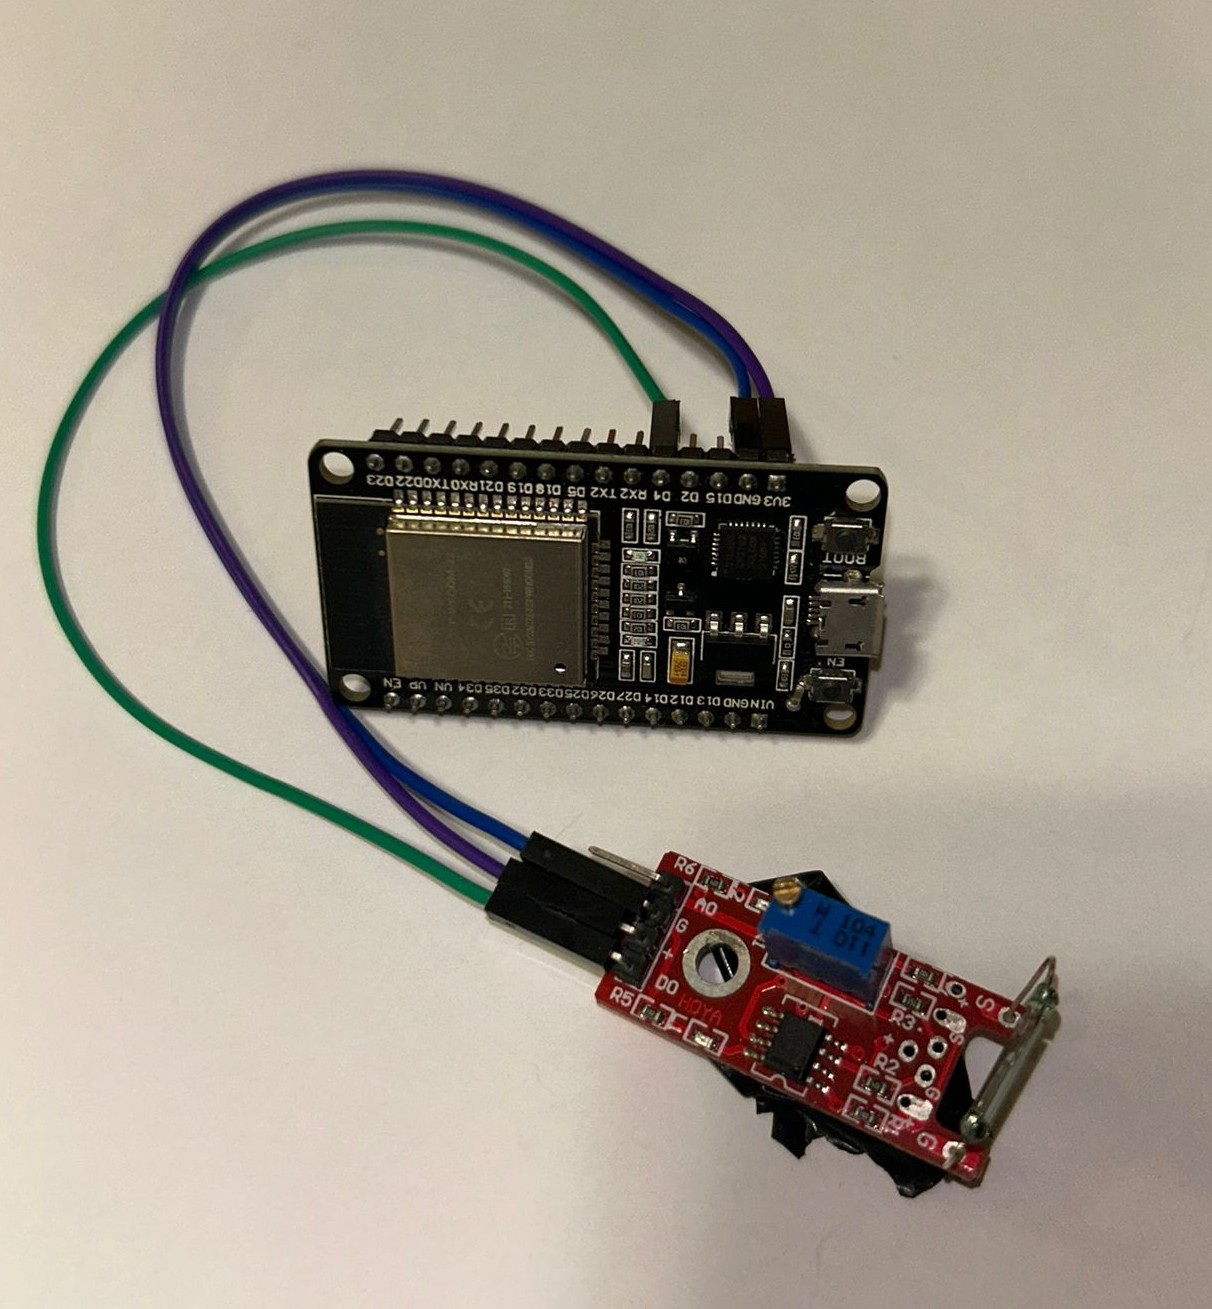
\includegraphics[width=\textwidth]{Img/nodo_puerta.jpg}
        \caption{Módulo de Puerta ($N_3$)}
        \label{fig:usr_nodo_puerta}
    \end{subfigure}
    \caption{Componentes de hardware y nodos sensores instalados en la habitación.}
    \label{fig:usr_nodos}
\end{figure}

\begin{enumerate}
    \item \textbf{Módulo de Ambiente ($N_1$):} mide la temperatura, la humedad y el nivel de ruido. Debe ubicarse en una zona de la pared libre de corrientes directas de aire acondicionado o calefactores. Incluye el interruptor electrónico que controla la corriente del enchufe general.
    \item \textbf{Módulo de Escritorio ($N_2$):} integra el sensor de presencia por radar y el fotorresistor de luminosidad. Debe colocarse sobre la mesa de trabajo, orientado diagonalmente hacia la silla del usuario a una distancia recomendada de entre 0.5 y 1.5 metros, asegurando que no haya objetos móviles interponiéndose (como aspas de ventiladores o cortinas).
    \item \textbf{Módulo de Puerta ($N_3$):} contiene el sensor magnético de contacto Reed. Se instala directamente sobre la hoja y el marco de la puerta de entrada para registrar los eventos físicos de apertura y cierre.
\end{enumerate}

Para que estos módulos se puedan comunicar con la red Wi-Fi y con el servidor central, es necesario programar los microcontroladores (las placas ESP32) por primera vez cargándoles su correspondiente software. Este proceso se gestiona de forma centralizada y visual desde la herramienta \textbf{ESPHome}, partiendo de la base de que ya disponemos de la Raspberry Pi en funcionamiento con Docker y los contenedores de \textbf{Home Assistant}, \textbf{ESPHome} y \textbf{Portainer} activos.

A continuación, se detalla el procedimiento que debe seguir el administrador o instalador para preparar y cargar el código en los módulos:
\begin{enumerate}
    \item \textbf{Acceder al panel de administración de ESPHome:} desde un ordenador conectado a la red local, abre el navegador de internet e introduce la dirección web del panel de ESPHome (habitualmente \texttt{http://ip\_raspberry\_pi:6052}, donde \texttt{ip\_raspberry\_pi} representa la dirección IP que proporciona Tailscale para tu Raspberry Pi). También puedes acceder a esta interfaz directamente desde la barra lateral izquierda de Home Assistant si está integrada.
    \item \textbf{Crear o seleccionar el dispositivo:} en la pantalla principal de ESPHome, haz clic en el botón ``+ Add Device'' para crear un nuevo dispositivo (o selecciona uno ya configurado de la lista). Dale un nombre descriptivo al módulo (ej. \texttt{nodo-ambiente}, \texttt{nodo-escritorio} o \texttt{nodo-puerta}).
    \item \textbf{Escribir la configuración de red y código:} introduce el código de configuración del módulo en formato de texto (los códigos específicos y completos para cada uno de los tres módulos se detallan más adelante en el Apéndice B, ``Manual Técnico y de Código''). Dentro del archivo de configuración, asegúrate de escribir correctamente los datos de tu red Wi-Fi:
    \begin{itemize}
        \item Nombre de la red Wi-Fi (\texttt{ssid}).
        \item Contraseña de la red Wi-Fi (\texttt{password}).
        \item Dirección IP fija asignada a ese módulo en concreto (para evitar conflictos de red y asegurar un acceso rápido).
    \end{itemize}
    \item \textbf{Conexión física y carga inicial del código:}
    Dado que es la primera vez que se programa la placa ESP32, la carga del software no puede hacerse de forma inalámbrica:
    \begin{enumerate}
        \item Conecta el módulo ESP32 físicamente mediante un cable micro-USB (o USB-C) a un puerto USB de tu ordenador, o bien directamente a uno de los puertos USB de la Raspberry Pi donde corre el sistema.
        \item En el panel de ESPHome, haz clic en el botón ``Install'' situado en la esquina superior derecha del dispositivo correspondiente.
        \item Si has conectado la placa a tu ordenador, selecciona la opción ``Plug into this computer'' (esta opción utiliza una tecnología del navegador Google Chrome o Edge para programarla directamente desde la web). Si has conectado la placa directamente a la Raspberry Pi, selecciona ``Plug into the server''.
        \item Haz clic en ``Install'' y espera a que el sistema compile el código y lo grabe en la placa (el proceso tardará un par de minutos y verás un registro de texto indicando el avance).
    \end{enumerate}
    \item \textbf{Instalación en ubicación definitiva y encendido:}
    Una vez programado con éxito el módulo por USB, ya puedes desconectarlo físicamente. A partir de este momento:
    \begin{enumerate}
        \item Coloca el módulo en su ubicación física recomendada en la estancia.
        \item Enchúfalo a una toma de corriente convencional utilizando cualquier cargador doméstico de móvil de $5\,\text{V}$ y un cable USB.
        \item Al recibir corriente, el microcontrolador iniciará de forma automática el software cargado, se conectará a la red Wi-Fi de tu casa y establecerá comunicación cifrada y segura con el servidor central para empezar a enviar lecturas.
    \end{enumerate}
    \item \textbf{Actualizaciones inalámbricas posteriores (OTA):} en el futuro, si necesitas hacer cualquier modificación en el comportamiento o los filtros del sensor, no tendrás que volver a conectar físicamente el módulo por USB. Podrás hacer las actualizaciones de forma inalámbrica por el aire seleccionando la opción ``Wirelessly'' dentro del menú ``Install'' de ESPHome.
\end{enumerate}

\subsection{Conexión y cableado de periféricos}
\label{sec:conexion_perifericos}

Para facilitar el ensamblado físico de los nodos sensores, se detallan a continuación los diagramas de cableado desarrollados con la herramienta de diseño electrónico \textbf{Fritzing}. En estos diagramas se representa de forma visual la placa de desarrollo ESP32, los sensores y actuadores asociados y la distribución de cables puente (Dupont) utilizando el código de colores estándar para alimentación ($5\,\text{V}$ en rojo, $3.3\,\text{V}$ en naranja, tierra o GND en negro) y líneas de datos (azul, amarillo o verde).

Al realizar las conexiones, es de vital importancia asegurar que los sensores compartan una masa común (GND) con el microcontrolador y que los niveles lógicos de entrada no superen la tolerancia máxima de $3.3\,\text{V}$ en los pines GPIO del ESP32.

\subsubsection{Cableado del Módulo de Ambiente (Nodo 1)}
El Módulo de Ambiente monitoriza variables higrométricas, iluminancia y nivel acústico de la estancia, además de controlar un relé optoacoplado. Las conexiones lógicas y de alimentación son las siguientes:
\begin{itemize}
    \item \textbf{Sensor DHT11 (Clima):} se alimenta a $3.3\,\text{V}$ (pin 3V3) y tierra (GND). Su pin de datos se conecta al \textbf{GPIO 4} del ESP32.
    \item \textbf{Fotorresistor LDR (Divisor de tensión):} se alimenta a $3.3\,\text{V}$ y GND. La salida analógica del divisor de tensión se conecta al canal ADC \textbf{GPIO 32} del ESP32.
    \item \textbf{Sensor de sonido KY-037 (Big Sound):} se alimenta a la línea de $5\,\text{V}$ (VIN) y GND para asegurar el correcto funcionamiento del comparador analógico. Su pin de salida digital (DO) se conecta al \textbf{GPIO 27} del ESP32.
    \item \textbf{Módulo de Relé (Control de enchufe):} se alimenta a $5\,\text{V}$ (VIN) y GND. Su pin de control (IN) se conecta al \textbf{GPIO 26} del ESP32.
\end{itemize}

En la Figura~\ref{fig:conexion_ambiente} se ilustra el conexionado completo del Nodo de Ambiente.

\begin{figure}[H]
    \centering
    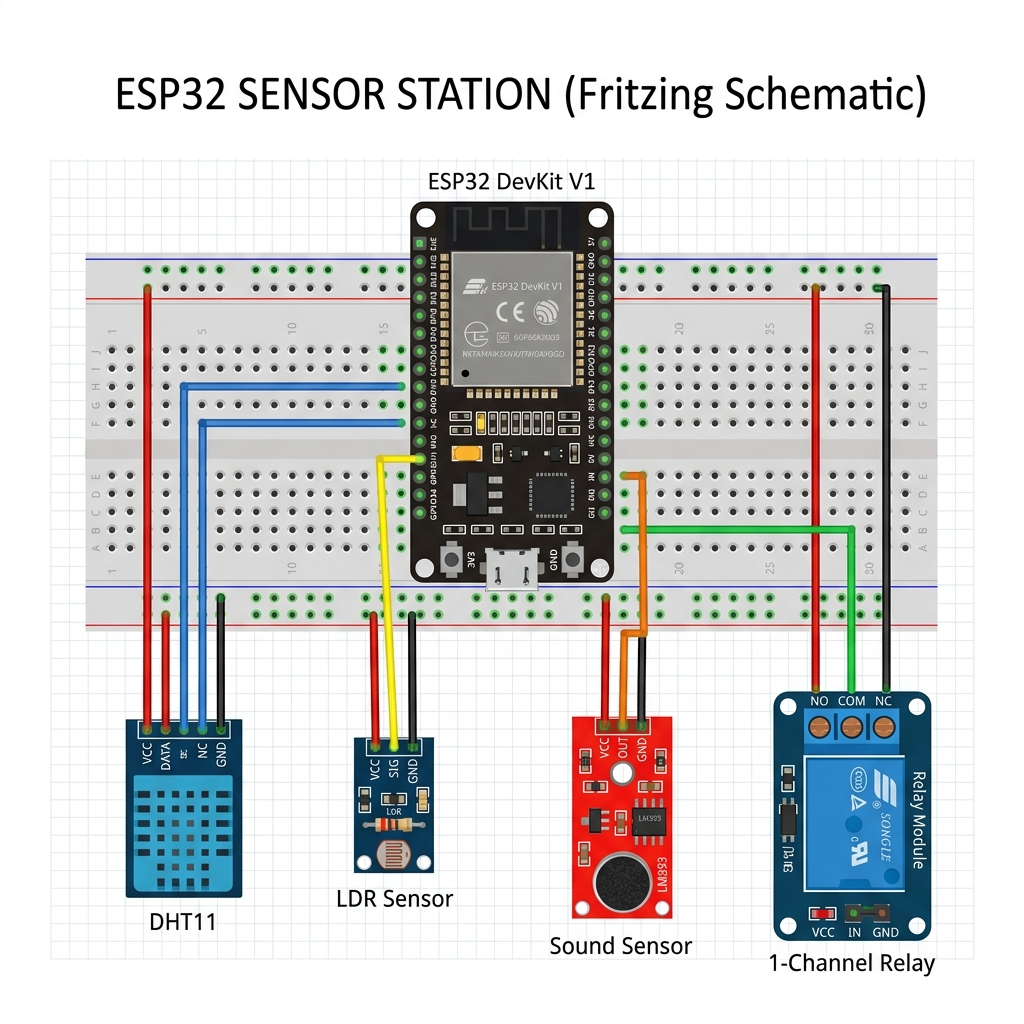
\includegraphics[width=0.65\textwidth]{Img/conexion_nodo_ambiente.png}
    \caption{Diagrama de conexionado de periféricos en Fritzing para el Módulo de Ambiente (Nodo 1).}
    \label{fig:conexion_ambiente}
\end{figure}

\subsubsection{Cableado del Módulo de Escritorio (Nodo 2)}
El Módulo de Escritorio integra el radar de microondas FMCW y el emisor láser. Su cableado se organiza de la siguiente manera:
\begin{itemize}
    \item \textbf{Radar mmWave HLK-LD2410C:} requiere una tensión de alimentación estable de $5\,\text{V}$ (VIN) y GND. La transmisión de datos se realiza a través de un canal serie UART cruzado: el pin de transmisión (TX) del radar se conecta al pin de recepción del ESP32 \textbf{RX2 (GPIO 16)}, y el pin de recepción (RX) del radar se conecta al pin de transmisión del ESP32 \textbf{TX2 (GPIO 17)}.
    \item \textbf{Módulo Emisor Láser KY-008:} se conecta directamente a la línea lógica \textbf{GPIO 12} del ESP32 para el control de encendido y apagado digital, y su pin de tierra a GND.
\end{itemize}

En la Figura~\ref{fig:conexion_escritorio} se muestra el conexionado correspondiente al Nodo de Escritorio.

\begin{figure}[H]
    \centering
    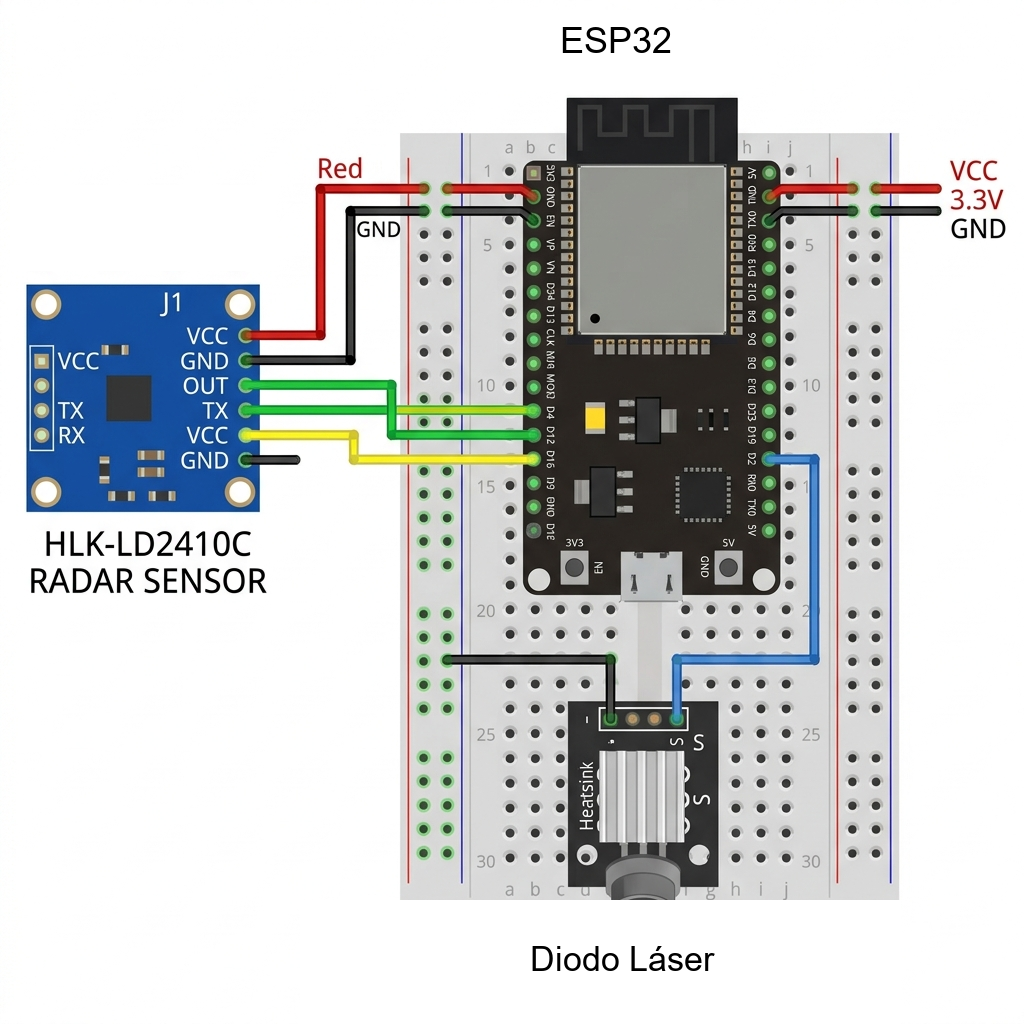
\includegraphics[width=0.65\textwidth]{Img/conexion_nodo_escritorio.png}
    \caption{Diagrama de conexionado de periféricos en Fritzing para el Módulo de Escritorio (Nodo 2).}
    \label{fig:conexion_escritorio}
\end{figure}

\subsubsection{Cableado del Módulo de Puerta (Nodo 3)}
El Módulo de Puerta monitoriza exclusivamente el acceso magnético de la puerta de entrada. Sus conexiones físicas son sumamente sencillas:
\begin{itemize}
    \item \textbf{Sensor Reed Switch (Contacto magnético):} se conecta directamente entre el pin \textbf{GPIO 4} del ESP32 y el pin de tierra (GND). Para simplificar el hardware y evitar el uso de resistencias físicas externas de acoplamiento, se aprovecha la resistencia de pull-up interna del microcontrolador, la cual se activa y configura mediante software.
\end{itemize}

En la Figura~\ref{fig:conexion_puerta} se ilustra el conexionado completo para el Módulo de Puerta.

\begin{figure}[H]
    \centering
    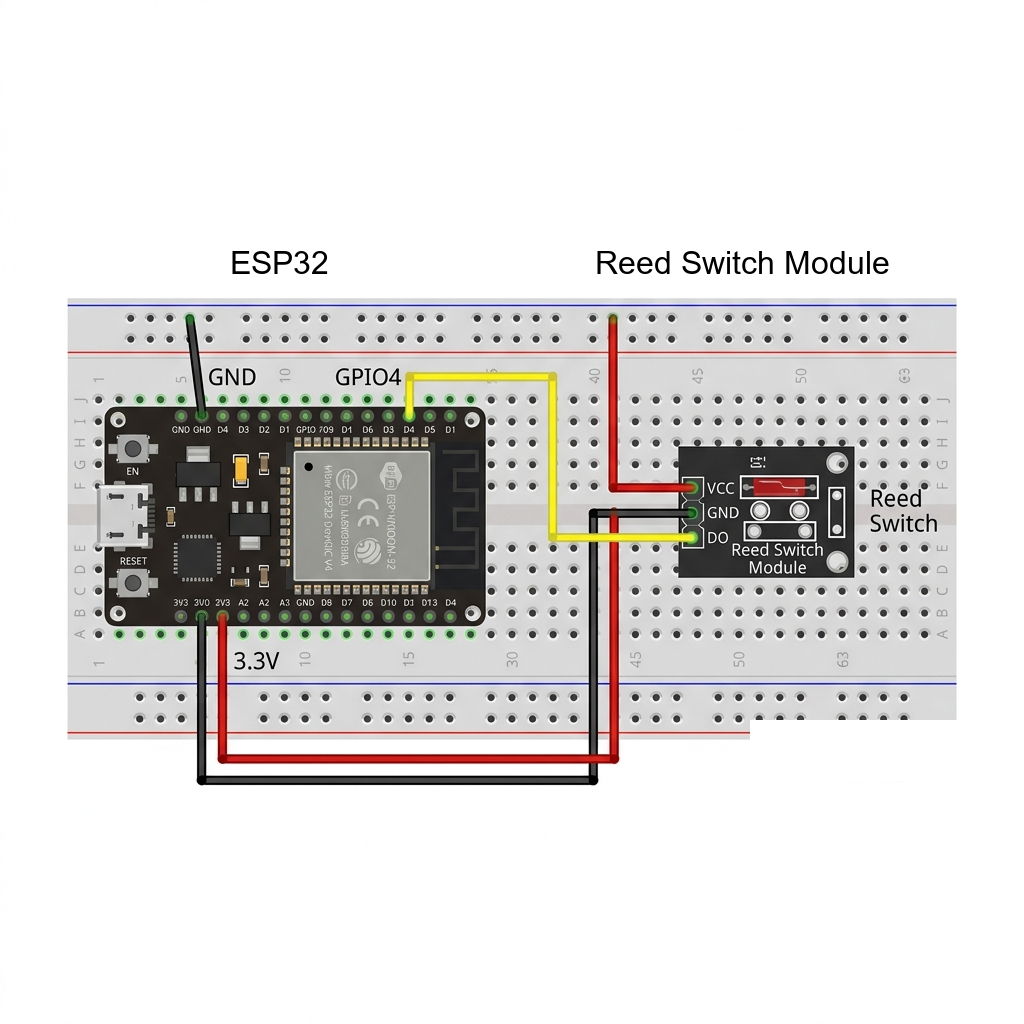
\includegraphics[width=0.65\textwidth]{Img/conexion_nodo_puerta.png}
    \caption{Diagrama de conexionado de periféricos en Fritzing para el Módulo de Puerta (Nodo 3).}
    \label{fig:conexion_puerta}
\end{figure}

\subsection{Manual de acceso y conexión}
Para ver el estado de la habitación y controlar las luces, puedes utilizar un ordenador, una tablet o tu teléfono móvil. Existen dos formas de conectarse dependiendo de dónde te encuentres:

\subsubsection{Acceso desde casa (Red Wi-Fi local)}
Si estás conectado a la misma red Wi-Fi de tu casa, el acceso es directo:
\begin{enumerate}
    \item Abre el navegador de internet que utilices habitualmente (Google Chrome, Safari, etc.) en tu ordenador o móvil.
    \item Introduce la dirección web que se te ha proporcionado para el sistema (habitualmente \texttt{http://192.168.1.150:8123}).
    \item Introduce tu nombre de usuario y tu contraseña.
\end{enumerate}

\subsubsection{Acceso desde fuera de casa (Conexión remota segura)}
Si estás en la calle, en el trabajo o de viaje, puedes seguir accediendo a tu sistema gracias a una red privada segura que conecta tu móvil directamente con tu casa:
\begin{enumerate}
    \item Instala la aplicación gratuita llamada \textbf{Tailscale} en tu teléfono móvil o en tu ordenador portátil (disponible en la tienda de aplicaciones de Android y Apple).
    \item Abre la aplicación Tailscale e inicia sesión con la cuenta de usuario que te haya configurado el administrador del sistema.
    \item Activa la conexión en la aplicación (deslizando el interruptor de encendido).
    \item Abre tu navegador de internet e introduce la misma dirección web que usas en casa. ¡Ya estarás conectado de forma segura!
\end{enumerate}

\subsection{Manual del panel de control (interfaz Lovelace)}
Una vez accedas, verás una pantalla organizada en tarjetas visuales muy intuitivas, diseñada para mostrarte toda la información de un solo vistazo (véase la Figura~\ref{fig:usr_dashboard1}):

\begin{figure}[H]
    \centering
    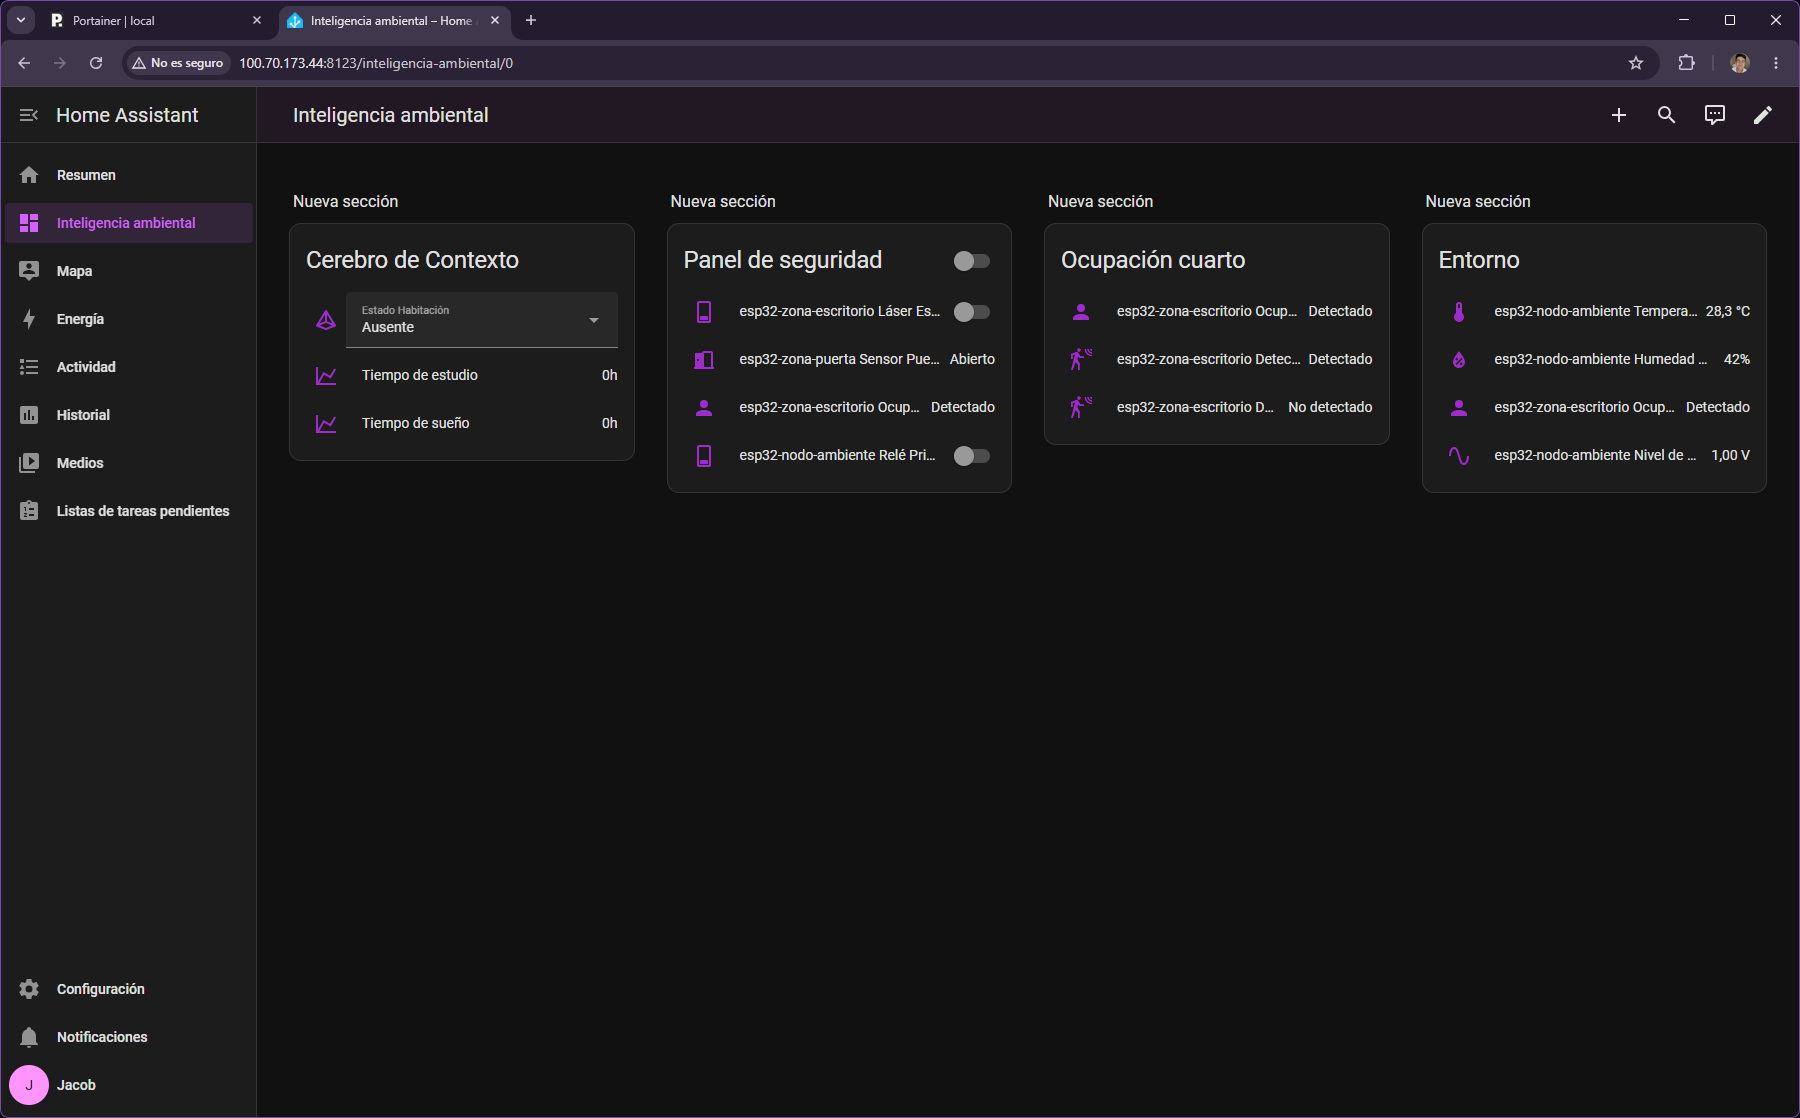
\includegraphics[width=0.90\textwidth]{Img/ha_dashboard_lovelace1.png}
    \caption{Pantalla principal del panel de control (Cuadro de Mandos Lovelace) en Home Assistant.}
    \label{fig:usr_dashboard1}
\end{figure}

\begin{itemize}
    \item \textbf{Interruptores de Control Manual:} en la parte superior verás botones para encender o apagar manualmente la luz de estudio del escritorio en cualquier momento, además de activar o desactivar la alarma del sistema.
    \item \textbf{Estado de Presencia:} la tarjeta central te muestra si hay alguien detectado en el escritorio o en la habitación en general. Gracias al radar de alta precisión, la pantalla te indicará si estás ``Sentado en Escritorio'', ``Descansando'' o si la habitación está ``Ausente''.
    \item \textbf{Mediciones del Entorno:} podrás ver de forma clara e instantánea la temperatura actual, el nivel de humedad y el nivel de ruido en la estancia.
    \item \textbf{Seguridad de Accesos:} indica si la puerta de la estancia está ``Abierta'' o ``Cerrada'', así como el estado del haz de luz de la barrera láser de la puerta.
    \item \textbf{Históricos y Gráficas de Actividad:} deslizando hacia la parte inferior del panel (o accediendo a la sección de históricos, Figura~\ref{fig:usr_dashboard2}), puedes revisar gráficas visuales que muestran cómo ha cambiado la temperatura a lo largo de las últimas horas, cuándo se abrió la puerta o a qué horas estuviste utilizando el escritorio.
\end{itemize}

\begin{figure}[H]
    \centering
    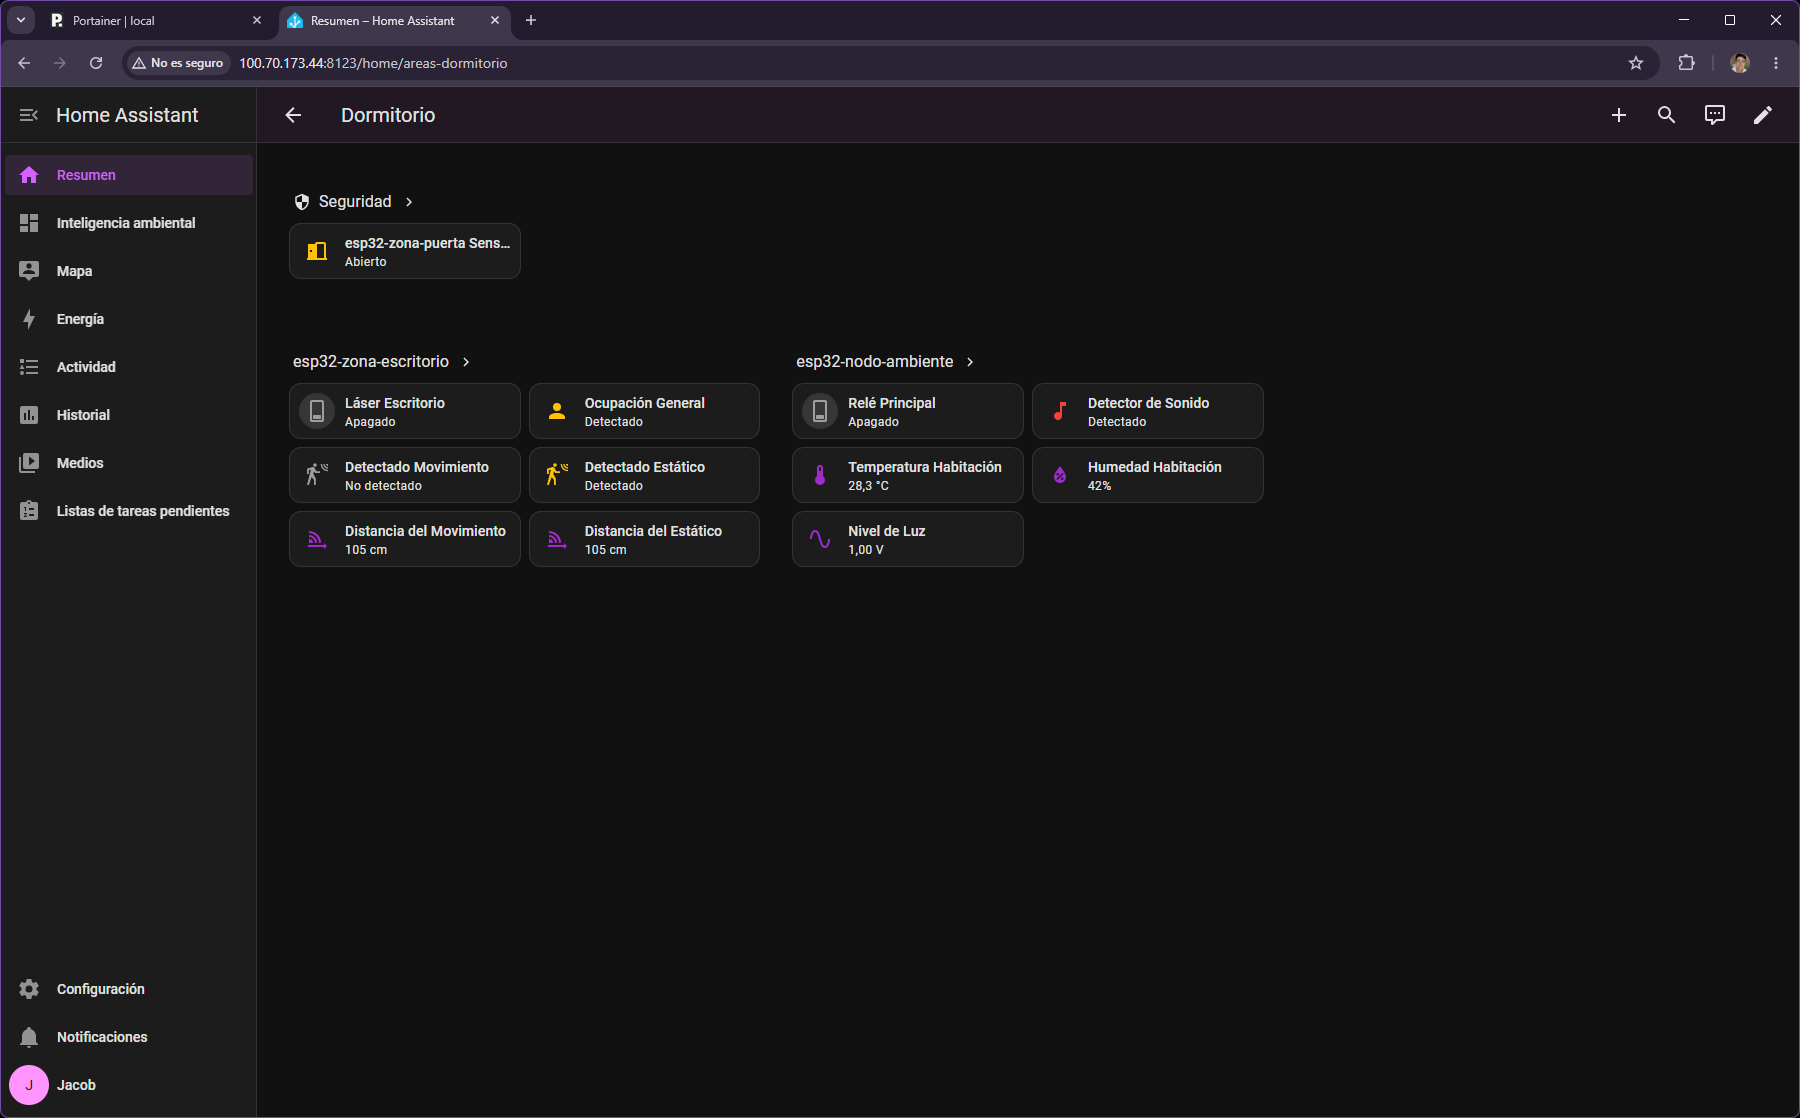
\includegraphics[width=0.90\textwidth]{Img/ha_dashboard_lovelace2.png}
    \caption{Sección de históricos y registros del panel de control.}
    \label{fig:usr_dashboard2}
\end{figure}

\subsection{Manual del comportamiento inteligente (automatizaciones)}
Para que no tengas que preocuparte de encender o apagar interruptores constantemente, el sistema ha sido programado con comportamientos automáticos inteligentes. A continuación te explicamos cómo funcionan:

\begin{enumerate}
    \item \textbf{Control automático de la luz del escritorio:}
    Cuando entres a la estancia y te sientes en la silla del escritorio, el sistema lo detectará al instante. Si es de noche o hay poca luz natural en la habitación, la luz del escritorio se encenderá automáticamente para que trabajes con comodidad. Al levantarte e irte del escritorio, la luz se apagará sola transcurridos unos instantes para ahorrar energía.
    
    \item \textbf{Avisos de descanso saludables (Método Pomodoro):}
    Pasar muchas horas seguidas sentado es perjudicial para la salud. Por ello, si el sistema de radar detecta que llevas más de 25 minutos seguidos sentado en el escritorio, la luz del escritorio realizará un parpadeo en color naranja y recibirás un mensaje de aviso en tu teléfono móvil indicándote que es hora de levantarte, beber agua y estirar las piernas durante un breve descanso de 5 minutos.
    
    \item \textbf{Sistema de alarma de la habitación:}
    Cuando vayas a salir de casa, puedes activar el ``Modo Alarma'' desde el panel de control en tu móvil. Si alguien abre la puerta de la habitación o cruza el haz de luz láser mientras la alarma está activa, el sistema lo considerará una intrusión: la luz de la habitación parpadeará en color rojo para alertar visualmente y recibirás una notificación de emergencia inmediata en tu teléfono móvil con el aviso.
    
    \item \textbf{Ahorro de energía automático (Modo Noche y Ausencia):}
    Si sales de la habitación y el sistema no detecta ningún movimiento ni respiración durante 10 minutos, apagará de forma automática todas las luces y aparatos eléctricos. De igual forma, si te vas a dormir y activas el ``Modo Noche'', el sistema apagará instantáneamente todos los equipos para asegurar tu descanso y evitar consumos innecesarios.
\end{enumerate}

\subsection{Guía de resolución de incidencias}
Esta sección recopila los problemas más comunes divididos en función del perfil de uso, facilitando tanto el diagnóstico rápido por parte del usuario final como la resolución de fallos lógicos o físicos de despliegue por parte del instalador.

\subsubsection{Incidencias de uso cotidiano (usuario final)}
A continuación, se describen los problemas relacionados con la operación y uso ordinario del sistema:

\begin{itemize}
    \item \textbf{La luz del escritorio no se enciende sola cuando me siento:}
    \begin{enumerate}
        \item Comprueba si hay suficiente luz natural en la habitación. Recuerda que el sistema está configurado para no encender la luz si la estancia ya está suficientemente iluminada por el sol.
        \item Asegúrate de que la lámpara esté enchufada al módulo de corriente y que el interruptor físico propio de la lámpara esté en posición de encendido.
    \end{enumerate}
    
    \item \textbf{En la pantalla aparece que un sensor no está disponible:}
    \begin{enumerate}
        \item Verifica que el módulo sensor en cuestión ($N_1$, $N_2$ o $N_3$) esté conectado a su cargador y que el cargador esté bien enchufado a la toma de corriente.
        \item Si el módulo está encendido, es posible que haya habido un corte temporal en la conexión Wi-Fi de tu casa. El dispositivo volverá a conectarse solo automáticamente una vez la red Wi-Fi se estabilice.
    \end{enumerate}
    
    \item \textbf{No puedo acceder al panel de control desde fuera de casa:}
    \begin{enumerate}
        \item Asegúrate de tener conexión a internet en tu móvil (datos móviles o Wi-Fi externo).
        \item Comprueba que tienes la aplicación \textbf{Tailscale} abierta y que el interruptor principal de conexión dentro de la aplicación esté activo.
    \end{enumerate}
\end{itemize}

\subsubsection{Incidencias de instalación y configuración (administrador/instalador)}
Esta sección aborda problemas específicos que pueden surgir durante el montaje de hardware, la programación de las placas o el despliegue del servidor central:

\begin{itemize}
    \item \textbf{El microcontrolador ESP32 no es reconocido por el ordenador al conectarlo por USB:}
    \begin{enumerate}
        \item \textbf{Causa:} Falta del controlador del puente USB-a-UART en el sistema operativo del ordenador. Las placas de desarrollo ESP32 comerciales suelen integrar chips conversores como el CP2102 de Silicon Labs o el CH340 de WCH.
        \item \textbf{Solución:} Descarga e instala los controladores oficiales del fabricante del chip (Silicon Labs CP210x USB to UART Bridge VCP Drivers o WCH CH340 Driver) correspondientes al sistema operativo utilizado (Windows, macOS o Linux).
        \item \textbf{Verificación:} Conecta de nuevo el microcontrolador y verifica que se asigne un puerto COM (en Windows) o un dispositivo de terminal virtual (en macOS/Linux, como \texttt{/dev/ttyUSB0}).
    \end{enumerate}

    \item \textbf{La Raspberry Pi 4 se queda colgada o se reinicia durante la compilación del código en ESPHome:}
    \begin{enumerate}
        \item \textbf{Causa:} Sobrecarga extrema de CPU y memoria RAM. El compilador de C++ integrado en ESPHome consume una gran cantidad de recursos, lo que puede agotar la memoria de la Raspberry Pi (especialmente en modelos de 1\,GB o 2\,GB de RAM o bajo configuraciones sin memoria de intercambio (\textit{swap})).
        \item \textbf{Solución A (Compilación local en PC):} Abre ESPHome, selecciona el menú de tres puntos del nodo y haz clic en ``Manual Download'' para compilar el firmware utilizando los recursos del ordenador local. Una vez descargado el archivo ejecutable compilado (\texttt{.bin}), utiliza el cargador web oficial de ESPHome (\texttt{https://web.esphome.io}) o la herramienta gráfica ESPHome Flasher desde el ordenador para grabar el código directamente en la placa ESP32 por USB.
        \item \textbf{Solución B (Optimización en la Raspberry Pi):} Configura un archivo de intercambio (\textit{swapfile}) de al menos 1\,GB en Raspberry Pi OS para dar soporte a la memoria RAM física en tareas de compilación intensa.
    \end{enumerate}

    \item \textbf{Inestabilidad general en la Raspberry Pi, apagados aleatorios o falta de detección de periféricos USB:}
    \begin{enumerate}
        \item \textbf{Causa:} Alimentación eléctrica deficiente. La Raspberry Pi 4 requiere una fuente de alimentación estable de $5\,\text{V}$ y un mínimo de $3\,\text{A}$ ($15\,\text{W}$). El uso de cargadores de móvil genéricos, cables USB de mala calidad o puertos USB de ordenador suele provocar caídas de tensión. Esto impide el correcto funcionamiento de componentes internos o de dispositivos conectados (como discos externos o módulos USB).
        \item \textbf{Solución:} Sustituye la fuente de alimentación por el adaptador oficial de corriente de la Raspberry Pi 4 o un cargador certificado compatible que garantice una salida dedicada de $5.1\,\text{V}$ y $3.0\,\text{A}$.
    \end{enumerate}

    \item \textbf{Los nodos ESP32 no logran conectarse a la red inalámbrica Wi-Fi:}
    \begin{enumerate}
        \item \textbf{Causa:} Incompatibilidad de banda de frecuencia de red. Los microcontroladores basados en el SoC ESP32 solo son compatibles con la banda de $2.4\,\text{GHz}$. Si el enrutador de acceso doméstico trabaja únicamente en la banda de $5\,\text{GHz}$ o tiene activo un sistema híbrido de autogestión de banda (Smart Connect) que obliga al nodo a enlazarse en $5\,\text{GHz}$, la conexión fallará.
        \item \textbf{Solución:} Accede al panel de configuración del enrutador y asegúrate de que la banda de $2.4\,\text{GHz}$ esté habilitada con un canal específico. Si el sistema híbrido da problemas, es recomendable configurar una red Wi-Fi virtual (SSID secundario) dedicada en exclusiva a dispositivos IoT forzada a operar en $2.4\,\text{GHz}$.
    \end{enumerate}

    \item \textbf{Las entidades de los nodos sensores aparecen en Home Assistant como ``No disponibles'':}
    \begin{enumerate}
        \item \textbf{Causa:} Desajuste en la clave de cifrado de la API o problemas de enrutamiento de red local.
        \item \textbf{Solución:} Abre el archivo de configuración del nodo en el panel de ESPHome y comprueba la clave de la API en la sección \texttt{api: encryption: key}. Verifica que esta clave de seguridad sea idéntica a la que introdujiste en la integración de Home Assistant. Si la clave es correcta, asegúrate de que la Raspberry Pi y las placas ESP32 se encuentren en la misma subred de red local y que los puertos de comunicación (por defecto, puerto TCP \texttt{6053}) no estén bloqueados por políticas de aislamiento de red del router.
    \end{enumerate}
\end{itemize}
